% ============================================================
% Question Bank: ch08-02 Making Inferences from Random Samples
% Topic Title: Making Inferences from Random Samples
% CCSS: 7.SP.A.2
% Questions: 27 (15 MC + 6 SA + 6 Graphical)
% ============================================================

% --- Multiple Choice Questions (15) ---

\begin{practiceQuestion}{8-2-q01}{mc}
\begin{questionText}
A random sample of $30$ apples from an orchard has a mean weight of $6.2$ ounces. What is the best prediction for the mean weight of all apples in the orchard?
\end{questionText}
\choiceA{Exactly $6.2$ ounces}
\choiceB{Approximately $6.2$ ounces}
\choiceC{More than $6.2$ ounces}
\choiceD{Less than $6.2$ ounces}
\correctAnswer{B}
\explanation{A random sample mean is a good estimate of the population mean. Because of natural sampling variability, we say the population mean is approximately — not exactly — $6.2$ ounces.}
\end{practiceQuestion}

\begin{practiceQuestion}{8-2-q02}{mc}
\begin{questionText}
In a random sample of $40$ students at a school, $14$ said they walk to school. If the school has $600$ students, how many are predicted to walk to school?
\end{questionText}
\choiceA{$14$}
\choiceB{$140$}
\choiceC{$210$}
\choiceD{$240$}
\correctAnswer{C}
\explanation{The sample proportion is $\frac{14}{40} = 0.35$. Multiply by the population: $0.35 \times 600 = 210$ students.}
\end{practiceQuestion}

\begin{practiceQuestion}{8-2-q03}{mc}
\begin{questionText}
A farmer takes four random samples of $25$ tomatoes and finds the mean weights are $5.1$, $5.4$, $4.9$, and $5.0$ ounces. What is the best estimate for the population mean weight?
\end{questionText}
\choiceA{$5.0$ ounces}
\choiceB{$5.1$ ounces}
\choiceC{$5.4$ ounces}
\choiceD{$4.9$ ounces}
\correctAnswer{B}
\explanation{Average the four sample means: $\frac{5.1 + 5.4 + 4.9 + 5.0}{4} = \frac{20.4}{4} = 5.1$ ounces. Averaging multiple samples gives a more reliable estimate.}
\end{practiceQuestion}

\begin{practiceQuestion}{8-2-q04}{mc}
\begin{questionText}
A pet store surveys $20$ randomly chosen customers. Eight customers own at least one cat. If the store has $350$ customers per month, predict how many own at least one cat.
\end{questionText}
\choiceA{$70$}
\choiceB{$140$}
\choiceC{$175$}
\choiceD{$280$}
\correctAnswer{B}
\explanation{The sample proportion is $\frac{8}{20} = 0.4$. Multiply: $0.4 \times 350 = 140$ customers.}
\end{practiceQuestion}

\begin{practiceQuestion}{8-2-q05}{mc}
\begin{questionText}
Which strategy most improves the reliability of a prediction about a population?
\end{questionText}
\choiceA{Using one very large convenience sample}
\choiceB{Taking multiple random samples and averaging the results}
\choiceC{Asking volunteers to respond}
\choiceD{Using the result from a single random sample}
\correctAnswer{B}
\explanation{Taking multiple random samples and averaging reduces the effect of random variation, giving a more reliable estimate of the population parameter.}
\end{practiceQuestion}

\begin{practiceQuestion}{8-2-q06}{mc}
\begin{questionText}
A candy company claims its bags contain an average of $50$ candies. A random sample of $15$ bags has a mean of $47$ candies. What can you infer?
\end{questionText}
\choiceA{The company's claim is certainly wrong}
\choiceB{The sample suggests the actual average may be lower than claimed}
\choiceC{The sample is too small to draw any conclusion}
\choiceD{The sample proves the average is exactly $47$}
\correctAnswer{B}
\explanation{The sample mean of $47$ is less than the claimed $50$. While one sample cannot prove the claim wrong, it suggests the actual average may be lower.}
\end{practiceQuestion}

\begin{practiceQuestion}{8-2-q07}{mc}
\begin{questionText}
Three random samples each contain $30$ students. Their mean math scores are $82$, $79$, and $84$. Another researcher takes one sample of $30$ and gets $75$. Which best estimates the population mean?
\end{questionText}
\choiceA{$75$}
\choiceB{$79$}
\choiceC{$81.67$}
\choiceD{$80$}
\correctAnswer{D}
\explanation{Average all four sample means: $\frac{82 + 79 + 84 + 75}{4} = \frac{320}{4} = 80$. Using all available samples gives the most reliable estimate.}
\end{practiceQuestion}

\begin{practiceQuestion}{8-2-q08}{mc}
\begin{questionText}
A random sample of $50$ bottles from a water plant had a mean volume of $16.1$ fluid ounces. The target volume is $16.0$ fluid ounces. A second random sample of $50$ bottles had a mean of $15.9$ fluid ounces. What is the best estimate of the population mean?
\end{questionText}
\choiceA{$15.9$ fl oz}
\choiceB{$16.0$ fl oz}
\choiceC{$16.1$ fl oz}
\choiceD{$32.0$ fl oz}
\correctAnswer{B}
\explanation{Average the two sample means: $\frac{16.1 + 15.9}{2} = 16.0$ fluid ounces. This estimate is close to the target volume.}
\end{practiceQuestion}

\begin{practiceQuestion}{8-2-q09}{mc}
\begin{questionText}
In a random sample of $25$ seventh graders, $10$ prefer vanilla ice cream. In a second random sample of $25$, $8$ prefer vanilla. If the grade has $200$ students, what is the best prediction for the number who prefer vanilla?
\end{questionText}
\choiceA{$18$}
\choiceB{$36$}
\choiceC{$72$}
\choiceD{$80$}
\correctAnswer{C}
\explanation{Average the two proportions: $\frac{10+8}{50} = \frac{18}{50} = 0.36$. Multiply: $0.36 \times 200 = 72$ students.}
\end{practiceQuestion}

\begin{practiceQuestion}{8-2-q10}{mc}
\begin{questionText}
A bakery sells an average of $120$ croissants per day. A random sample of $5$ days shows sales of $115$, $128$, $110$, $125$, and $122$. The sample mean is:
\end{questionText}
\choiceA{$115$}
\choiceB{$120$}
\choiceC{$122$}
\choiceD{$125$}
\correctAnswer{B}
\explanation{Add the values: $115 + 128 + 110 + 125 + 122 = 600$. Divide by $5$: $\frac{600}{5} = 120$.}
\end{practiceQuestion}

\begin{practiceQuestion}{8-2-q11}{mc}
\begin{questionText}
A biologist counts the number of frogs in $5$ randomly selected ponds. The counts are $12$, $18$, $15$, $20$, and $10$. If there are $40$ similar ponds in the region, predict the total number of frogs.
\end{questionText}
\choiceA{$300$}
\choiceB{$400$}
\choiceC{$600$}
\choiceD{$750$}
\correctAnswer{C}
\explanation{Mean per pond: $\frac{12+18+15+20+10}{5} = \frac{75}{5} = 15$. Multiply by $40$ ponds: $15 \times 40 = 600$ frogs.}
\end{practiceQuestion}

\begin{practiceQuestion}{8-2-q12}{mc}
\begin{questionText}
Two students each take a random sample of $20$ classmates. Student A finds $60\%$ prefer pizza; Student B finds $50\%$ prefer pizza. The most likely reason for the difference is:
\end{questionText}
\choiceA{One of the samples is biased}
\choiceB{Natural variability between random samples}
\choiceC{The population preference changed between samples}
\choiceD{One student made a calculation error}
\correctAnswer{B}
\explanation{Random samples naturally produce different results because they include different members of the population. This variation is expected and does not indicate bias.}
\end{practiceQuestion}

\begin{practiceQuestion}{8-2-q13}{mc}
\begin{questionText}
A random sample of $60$ households in a city shows an average of $1.8$ cars per household. The city has $15{,}000$ households. Predict the total number of cars.
\end{questionText}
\choiceA{$1{,}080$}
\choiceB{$10{,}800$}
\choiceC{$27{,}000$}
\choiceD{$30{,}000$}
\correctAnswer{C}
\explanation{Multiply the sample mean by the number of households: $1.8 \times 15{,}000 = 27{,}000$ cars.}
\end{practiceQuestion}

\begin{practiceQuestion}{8-2-q14}{mc}
\begin{questionText}
A researcher takes three random samples of students and records the percentage who participate in a sport: $42\%$, $38\%$, and $44\%$. The researcher wants a single estimate. What should she use?
\end{questionText}
\choiceA{The highest percentage, $44\%$}
\choiceB{The lowest percentage, $38\%$}
\choiceC{The average of the three, about $41.3\%$}
\choiceD{The median, $42\%$}
\correctAnswer{C}
\explanation{Average the three results: $\frac{42 + 38 + 44}{3} = \frac{124}{3} \approx 41.3\%$. Averaging multiple samples provides a more reliable estimate than using any single result.}
\end{practiceQuestion}

\begin{practiceQuestion}{8-2-q15}{mc}
\begin{questionText}
A sample of $50$ packages from a shipping company has a mean weight of $4.5$ pounds. If the company ships $2{,}000$ packages per day, predict the total weight shipped daily.
\end{questionText}
\choiceA{$4{,}500$ pounds}
\choiceB{$9{,}000$ pounds}
\choiceC{$225$ pounds}
\choiceD{$100{,}000$ pounds}
\correctAnswer{B}
\explanation{Multiply the sample mean by the number of packages: $4.5 \times 2{,}000 = 9{,}000$ pounds.}
\end{practiceQuestion}

% --- Short Answer Questions (6) ---

\begin{practiceQuestion}{8-2-q16}{sa}
\begin{questionText}
In a random sample of $25$ students, $15$ said reading is their favorite hobby. If the school has $500$ students, predict how many prefer reading.
\end{questionText}
\correctAnswer{$300$}
\explanation{The sample proportion is $\frac{15}{25} = 0.6$. Multiply: $0.6 \times 500 = 300$ students.}
\end{practiceQuestion}

\begin{practiceQuestion}{8-2-q17}{sa}
\begin{questionText}
A farmer measures the heights of $10$ randomly selected corn stalks: $58$, $62$, $60$, $65$, $59$, $63$, $61$, $64$, $57$, and $61$ inches. What is the sample mean?
\end{questionText}
\correctAnswer{$61$}
\explanation{Add all values: $58+62+60+65+59+63+61+64+57+61 = 610$. Divide by $10$: $\frac{610}{10} = 61$ inches.}
\end{practiceQuestion}

\begin{practiceQuestion}{8-2-q18}{sa}
\begin{questionText}
Two random samples of $30$ students have mean quiz scores of $84$ and $88$. What is the best single estimate for the population mean?
\end{questionText}
\correctAnswer{$86$}
\explanation{Average the two sample means: $\frac{84 + 88}{2} = 86$. Using the mean of multiple samples provides a better estimate.}
\end{practiceQuestion}

\begin{practiceQuestion}{8-2-q19}{sa}
\begin{questionText}
A random sample of $20$ shoppers found that the mean amount spent was $\$45$. If the store has $800$ shoppers per weekend, predict the total spent by all weekend shoppers.
\end{questionText}
\correctAnswer{$\$36{,}000$}
\explanation{Multiply the sample mean by the number of shoppers: $\$45 \times 800 = \$36{,}000$.}
\end{practiceQuestion}

\begin{practiceQuestion}{8-2-q20}{sa}
\begin{questionText}
A random sample of $40$ eggs has a mean weight of $56$ grams. A second sample of $40$ eggs has a mean weight of $58$ grams. A third sample has a mean of $55$ grams. What is the best estimate of the population mean?
\end{questionText}
\correctAnswer{$56.3$ grams}
\explanation{Average the three sample means: $\frac{56 + 58 + 55}{3} = \frac{169}{3} \approx 56.3$ grams.}
\end{practiceQuestion}

\begin{practiceQuestion}{8-2-q21}{sa}
\begin{questionText}
A gym takes a random sample of $50$ members and finds that $30$ members attend at least $3$ times per week. If the gym has $1{,}200$ members, predict how many attend at least $3$ times per week.
\end{questionText}
\correctAnswer{$720$}
\explanation{The sample proportion is $\frac{30}{50} = 0.6$. Multiply: $0.6 \times 1{,}200 = 720$ members.}
\end{practiceQuestion}

% --- Graphical Questions (3 GMC + 3 GSA) ---

\begin{practiceQuestion}{8-2-q22}{gmc}
\begin{questionText}
A random sample of $20$ students was asked how many books they read last month. The dot plot shows the results.

\begin{center}
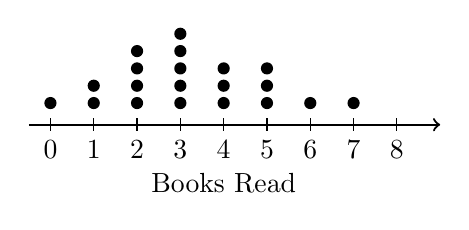
\begin{tikzpicture}[scale=0.55]
  \draw[thick,->] (-0.5,0) -- (9,0);
  \foreach \x in {0,...,8} \draw (\x,0.15) -- (\x,-0.15) node[below] {$\x$};
  \node[below] at (4,-0.9) {Books Read};
  % dots: 0(1), 1(2), 2(4), 3(5), 4(3), 5(3), 6(1), 7(1)
  \fill (0,0.5) circle (4pt);
  \foreach \y in {1,2} \fill (1,0.1+\y*0.4) circle (4pt);
  \foreach \y in {1,...,4} \fill (2,0.1+\y*0.4) circle (4pt);
  \foreach \y in {1,...,5} \fill (3,0.1+\y*0.4) circle (4pt);
  \foreach \y in {1,...,3} \fill (4,0.1+\y*0.4) circle (4pt);
  \foreach \y in {1,...,3} \fill (5,0.1+\y*0.4) circle (4pt);
  \fill (6,0.5) circle (4pt);
  \fill (7,0.5) circle (4pt);
\end{tikzpicture}
\end{center}

If the school has $300$ students, predict how many read $3$ or more books.
\end{questionText}
\choiceA{$65$}
\choiceB{$130$}
\choiceC{$195$}
\choiceD{$260$}
\correctAnswer{C}
\explanation{Count dots at $3$ or more: $5+3+3+1+1 = 13$ out of $20$. The proportion is $\frac{13}{20} = 0.65$. Multiply: $0.65 \times 300 = 195$ students.}
\end{practiceQuestion}

\begin{practiceQuestion}{8-2-q23}{gmc}
\begin{questionText}
Three random samples of $25$ animals at a shelter were weighed. The mean weights are shown in the table.

\begin{center}
\begin{tabular}{|c|c|}
\hline
\textbf{Sample} & \textbf{Mean Weight (lb)} \\
\hline
$1$ & $22$ \\
$2$ & $19$ \\
$3$ & $25$ \\
\hline
\end{tabular}
\end{center}

Which is the best estimate for the mean weight of all animals at the shelter?
\end{questionText}
\choiceA{$19$ lb}
\choiceB{$22$ lb}
\choiceC{$25$ lb}
\choiceD{$66$ lb}
\correctAnswer{B}
\explanation{Average the three sample means: $\frac{22+19+25}{3} = \frac{66}{3} = 22$ pounds.}
\end{practiceQuestion}

\begin{practiceQuestion}{8-2-q24}{gmc}
\begin{questionText}
A survey asked a random sample of $50$ families how many pets they own. The bar graph shows the results.

\begin{center}
\begin{tikzpicture}[scale=0.45]
  \draw[thick,->] (0,0) -- (0,11) node[above] {Families};
  \draw[thick,->] (0,0) -- (8.5,0);
  \foreach \y in {0,2,...,10} {
    \draw (-0.2,\y/2) -- (0,\y/2);
  }
  \foreach \y in {0,4,...,20} {
    \node[left=3pt] at (0,\y/2) {$\y$};
    \draw[gray!30] (0,\y/2) -- (8,\y/2);
  }
  \fill[funBlue!70] (0.5,0) rectangle (1.5,6);
  \fill[funBlue!70] (2.5,0) rectangle (3.5,10);
  \fill[funBlue!70] (4.5,0) rectangle (5.5,6);
  \fill[funBlue!70] (6.5,0) rectangle (7.5,3);
  \node[below] at (1,-0.3) {$0$};
  \node[below] at (3,-0.3) {$1$};
  \node[below] at (5,-0.3) {$2$};
  \node[below] at (7,-0.3) {$3+$};
  \node[below] at (4,-1.2) {Number of Pets};
\end{tikzpicture}
\end{center}

The bars show that $12$ families own $0$ pets, $20$ own $1$ pet, $12$ own $2$ pets, and $6$ own $3$ or more. If there are $800$ families in the town, predict how many own at least $1$ pet.
\end{questionText}
\choiceA{$320$}
\choiceB{$480$}
\choiceC{$608$}
\choiceD{$640$}
\correctAnswer{C}
\explanation{Families with at least $1$ pet: $20 + 12 + 6 = 38$ out of $50$. Proportion: $\frac{38}{50} = 0.76$. Multiply: $0.76 \times 800 = 608$ families.}
\end{practiceQuestion}

\begin{practiceQuestion}{8-2-q25}{gsa}
\begin{questionText}
The dot plot shows the number of hours $15$ randomly selected students spend on homework each night.

\begin{center}
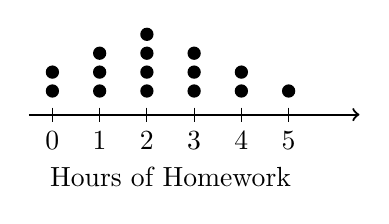
\begin{tikzpicture}[scale=0.6]
  \draw[thick,->] (-0.5,0) -- (6.5,0);
  \foreach \x in {0,...,5} \draw (\x,0.15) -- (\x,-0.15) node[below] {$\x$};
  \node[below] at (2.5,-0.9) {Hours of Homework};
  % 0(2), 1(3), 2(4), 3(3), 4(2), 5(1) = 15
  \foreach \y in {1,2} \fill (0,0.1+\y*0.4) circle (4pt);
  \foreach \y in {1,...,3} \fill (1,0.1+\y*0.4) circle (4pt);
  \foreach \y in {1,...,4} \fill (2,0.1+\y*0.4) circle (4pt);
  \foreach \y in {1,...,3} \fill (3,0.1+\y*0.4) circle (4pt);
  \foreach \y in {1,2} \fill (4,0.1+\y*0.4) circle (4pt);
  \fill (5,0.5) circle (4pt);
\end{tikzpicture}
\end{center}

What is the mean number of hours of homework per night for this sample?
\end{questionText}
\correctAnswer{$2.2$}
\explanation{Sum: $0(2)+1(3)+2(4)+3(3)+4(2)+5(1) = 0+3+8+9+8+5 = 33$. Divide by $15$: $\frac{33}{15} = 2.2$ hours.}
\end{practiceQuestion}

\begin{practiceQuestion}{8-2-q26}{gsa}
\begin{questionText}
The table shows the results of three random samples taken from a lake to estimate the fish population.

\begin{center}
\begin{tabular}{|c|c|c|}
\hline
\textbf{Sample} & \textbf{Fish Caught} & \textbf{Tagged Fish} \\
\hline
$1$ & $30$ & $6$ \\
$2$ & $30$ & $5$ \\
$3$ & $30$ & $7$ \\
\hline
\end{tabular}
\end{center}

A total of $90$ fish were originally tagged and released. Using the combined data from all three samples, estimate the total fish population in the lake.
\end{questionText}
\correctAnswer{$450$}
\explanation{In total, $6+5+7 = 18$ tagged fish were found in $90$ caught. The proportion of tagged fish is $\frac{18}{90} = \frac{1}{5}$. Set up: $\frac{90}{N} = \frac{1}{5}$, so $N = 90 \times 5 = 450$ fish.}
\end{practiceQuestion}

\begin{practiceQuestion}{8-2-q27}{gsa}
\begin{questionText}
A school surveyed two random samples of $25$ students each about their daily screen time. The results are shown.

\begin{center}
\begin{tabular}{|c|c|c|c|}
\hline
\textbf{Sample} & \textbf{Mean (hr)} & \textbf{0--2 hr} & \textbf{3+ hr} \\
\hline
$1$ & $2.8$ & $9$ & $16$ \\
$2$ & $3.2$ & $7$ & $18$ \\
\hline
\end{tabular}
\end{center}

If the school has $750$ students, use both samples to predict how many students have $3$ or more hours of daily screen time.
\end{questionText}
\correctAnswer{$510$}
\explanation{Combine: $16 + 18 = 34$ out of $50$ students have $3$+ hours. Proportion: $\frac{34}{50} = 0.68$. Multiply: $0.68 \times 750 = 510$ students.}
\end{practiceQuestion}
